\documentclass[tikz,border=5mm]{standalone}
\usepackage[T1]{fontenc}
\usepackage{fontspec}
\setmainfont{Fira Sans}[
  BoldFont=Fira Sans Bold,
  ItalicFont=Fira Sans Italic,
]
\usetikzlibrary{positioning, arrows.meta, shadows.blur, calc}

\definecolor{mTeal}{HTML}{2B7A78}
\definecolor{mBrown}{HTML}{C9956B}
\definecolor{mGray}{HTML}{888888}
\definecolor{mBg}{HTML}{FAFAFA}

\begin{document}
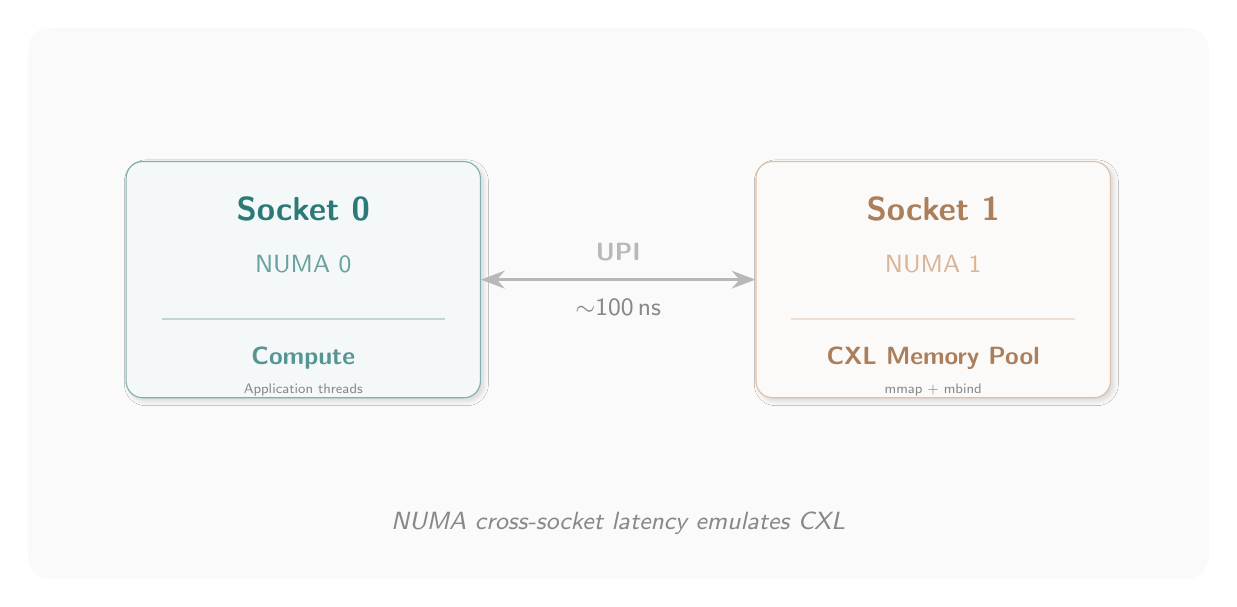
\begin{tikzpicture}[
  every node/.style={font=\sffamily},
  chip/.style={draw, rounded corners=6pt, minimum width=4.5cm,
               minimum height=3cm, align=center,
               blur shadow={shadow blur steps=8, shadow xshift=0.4mm,
               shadow yshift=-0.4mm, shadow opacity=15}},
  >=Stealth,
]
  \fill[mBg, rounded corners=8pt] (-7.5,-3.5) rectangle (7.5,3.5);

  % Socket 0
  \node[chip, draw=mTeal!60, fill=mTeal!5] (s0) at (-4,0.3) {};
  \node[mTeal, font=\sffamily\large\bfseries] at (-4, 1.2) {Socket 0};
  \node[mTeal!70, font=\sffamily\small] at (-4, 0.5) {NUMA 0};
  \draw[mTeal!30, thick] (-5.8,-0.2) -- (-2.2,-0.2);
  \node[mTeal!80, font=\sffamily\small\bfseries] at (-4,-0.7) {Compute};
  \node[mGray, font=\sffamily\tiny] at (-4,-1.1) {Application threads};

  % Socket 1
  \node[chip, draw=mBrown!60, fill=mBrown!5] (s1) at (4,0.3) {};
  \node[mBrown!85!black, font=\sffamily\large\bfseries] at (4, 1.2) {Socket 1};
  \node[mBrown!70, font=\sffamily\small] at (4, 0.5) {NUMA 1};
  \draw[mBrown!30, thick] (2.2,-0.2) -- (5.8,-0.2);
  \node[mBrown!85!black, font=\sffamily\small\bfseries] at (4,-0.7) {CXL Memory Pool};
  \node[mGray, font=\sffamily\tiny] at (4,-1.1) {mmap + mbind};

  % UPI interconnect
  \draw[{Stealth[length=3mm]}-{Stealth[length=3mm]}, very thick, mGray!60]
    (s0.east) -- (s1.west)
    node[midway, above=3pt, font=\sffamily\small\bfseries] {UPI}
    node[midway, below=3pt, font=\sffamily\small, mGray] {$\sim$100\,ns};

  % Tagline
  \node[mGray, font=\sffamily\itshape\small] at (0,-2.8)
    {NUMA cross-socket latency emulates CXL};
\end{tikzpicture}
\end{document}
